\documentclass[a4paper,12pt]{book}


\usepackage{preamble}

\begin{document}


\chapter{Definição do Problema}

\section{Problema do Caixeiro Viajante (TSP)}

	Um problema computacional bastante conhecido é o do caixeiro viajante: dado um conjunto de
cidades, que devem ser percorridas por um caixeiro, qual a rota que minimiza a distância a
percorrer?
	Um modo direto de resolução deste problema é analisar todas as possibilidades possiveis e
encontrar a com menor distância. Esta abordagem não é a mais aconselhavel uma vez que o número de
operações requeridas para tal cresce exponencialmente com o número de cidades a percorrer.

	Por este motivo se desenvolveu ao longo de varios anos métodos menos custosos para obter ou pelo
menos se aproximar da solução. Listaremos agora as estratégias mais comuns utilizadas

\begin{enumerate}
\item Vizinho mais próximo
\item Dois ótimo
\end{enumerate}


\section{Problema de roteamento de veículos}

	Uma extensão clara do problema do caixeiro viajante é o problema de roteamento de veículos: dado
um conjunto de entregas para clientes, que podem ser atendidos por mais que um veículo, qual o
melhor conjunto de rotas que miniza a distância total percorrida?

	A seguir especificaremos o problema matematicamente.

	Dado $C$ ( conjunto de clientes) tal que $C \subset \mathbb{R}^2$. O algoritmo $Alg(k,C)$
retorna o conjunto $f_i \in \mathbb{N}_i\times C$ de funções ( rotas) tal que $\sum_{i=1}^k\#
\mathbb{N}_i = \#C$ e $\cap_{i=1}^k \mathbb{N}_i= \emptyset$

	Existem algumas variações do problema de roteamento de veículos que serão listadas abaixo
\begin{enumerate}
\item Com carga (VRPC)
\item Com limite de tempo (VRPTW)
\item Com limite de veículos
\end{enumerate}


	Nosso problema é basicamente um VRP que busca minimizar o número de veículos utilizados e a
distância percorrida.



	Dado um conjunto de pontos em um plano devesse determinar a ordem a percorrer estes pontos de
modo a minimizar o custo do percurso.



\chapter{Algoritmos de Poupança}
\section{Clark and Wright}

 O algoritmo econômia de Clarke e Wright é uma das mais conhecidas heuristicas para VRP. Foi
desenvolvido em {\color{red} referenciar} e aplica-se a problemas para os quais o numero de veículo
não é fixo, e trabalha igualmente bem para problemas com digrafos e grafos. Quando duas rotas
$(0,\ldots, i, 0)$ e $(0,j,\ldots,0)$ podem possivelmente ser mescladas em uma rota simples
$(0,\ldots,i,j,\ldots,0)$, uma economia de distância $s_{ij}=c_{i0}+c_{0j}-c_{ij}$ é gerada. O
algoritmo trabalha como segue:

\begin{description}
\item[Step 1.] Savings computation

\begin{itemize}
\item Calcule o custo $s_{ij} = c_{i0}+c_{0j}-c_{ij}$ para $i,j=1,\ldots,n$ e $i\neq j$.
\item Crie $n$ rotas de veículos $(0,i,0)$ para $i=1,\ldots,n$.
\item Ordene as poupanças de modo não crescente ( Não é necessário )
\end{itemize}

\item[Step 2.] Melhor combinação possivel

Inicie do topo da lista de custos, executando o seguinte:

\begin{itemize}
\item Dada um custo $s_{ij}$, determine se há duas rotas que podem possivelmente ser mescladas:

\begin{itemize}
\item Uma iniciando com $(0,j)$
\item Uma terminando com $(0,i)$
\end{itemize}

\item Combine essas duas rotas deletando $(0,j)$ e $(0,i)$ e introduzindo $(i,j)$.
\end{itemize}
%
%\item[Step 2.] Extensão de Rotas (Versão Sequêncial)
%\begin{itemize}
%\item Considere uma volta de cada rota $(0,i,\ldots,j,0)$.
%\item Determine a primeira poupança $s_{ki}$ ou $s_{jl}$ que pode possivelmente ser usada para
%mesclar a rota atual com outra rota terminando com $(k,0)$ ou iniciando com $(0,l)$.
%\item Implemente a mescla e repetição dessa operação para a rota atual.
%\item Se não há mesclas possiveis, considere a próxima rota e reaplique a mesma operação.
%\item Pare quando a mesclagem de rotas não for possivel.
%\end{itemize}

\end{description}

\section{Emparelhamento baseado no algoritmo de poupança}

 Ista é uma modificação interessante para o algoritmo de poupança padrão ( descrições similares são
feitas por {\color{red} referênciar} e {\color{red} referênciar} onde em cada interação a poupança
$s_{ij}$ obtida por mesclar rotas $p$ e $q$ é calculado como $s_{ij} = t(S_i) + t(S_j) - t(S_i \cap
S_j)$, onde $S_k$ é o conjunto de vértices da rota k, e $t(S_k)$ é o comprimento de uma solução
ótima para o TSP em $S_k$.

 Um problema de emparelhamento sobre o conjunto $S_k$ é resolvido usando os $s_{ij}$ valores com
custo de emparelhamento, e as rotas correspondem à emparelhamento ótimo estão mescladas a
permanencia da fazibilidade.


\section{Algoritmo de melhoria para Mult-rota}

 Algoritmos de melhoria esforçam-se para atualizar alguma possivel solução executando um sequência
de mudançãs dos vertices e arestas dentro ou entre rotas de veículos. Heuristicas de melhoramento de
multi-rotas para VRP operão em cada rota de veículo tomando muitas rotas em um tempo(?). Podemos
encontrar descrições de mudanças de arestas para VRP nestas três referências:

\begin{itemize}
\item {\color{red} Referenciar}
\item {\color{red} Referenciar}
\item {\color{red} Referenciar}
\end{itemize}

 Thompson e Psaraftis (1993) propõem um método baseado nos conceitos de $k$-transferência ciclicas
que envolvem transferência de $k$ demandas da rota $I^j$ para a rota $I^{\delta(j)}$ para cada $j$ e
inteiro fixo $k$. O conjunto de rotas $\{ I^r \}$, com $r = 1, \ldots, m$, constitui um solução
possivel e $\delta$ é uma permutação cíclica de um subconjunto de $\{1, \ldots, m\}$. Em particular,
quando $\delta$ tem cardinalidade fixa $C$, obtemos um $C$-ciclo $k$-transferência. Permitindo $k$
demanda modelo em cada rota, transferência de demanda pode ser realizada através de permutações mais
que permutações ciclicas, Devido a complexidade das pesquisas de vizinhanças de transferências
cíclicas, é realizada heuristicamente. O operador de 3-ciclo 2-transferências é ilustrado na figura
abaixo.


\begin{figure}[!ht]
\centering
\includegraphics[width=10cm]{./fig/thompPsar.png}
\caption{O operador de transferência cíclica. A ideia base é transferir simultaneamente os clientes
denotados pelo ciclo branco de maneira ciclica entre as rotas. Mais precisamente aqui clientes $a$ e
$c$ na rota 1, $f$ e $j$ na rota 2 e $o$ e $p$ na rota 4 são transferidos simultaneamente para as
rotas 2, 4, e 1 respectivamente e a rota 3 permanece intocada.}
\end{figure}

\subsection{VAN BREEDAM'S ANALYSIS}

 Agora sumarizaremos a analise de Van Breedam's. Há quatro operações a considerar, as quais são:

\begin{enumerate}
\item String Cross (SC): Duas cadeias de vertices são mudadas pelo cruzamento de duas arestas de
diferêntes rotas.

\begin{figure}[!ht]
\centering
\includegraphics[width=10cm]{./fig/BreedSC.png}
\end{figure}

\item String Exchange (SE): Duas cadeias de no mínimo $k$ vértices são mudadas entre duas rotas.

\begin{figure}[!ht]
\centering
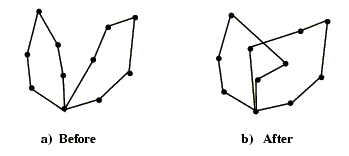
\includegraphics[width=10cm]{./fig/BreedSE.png}
\end{figure}

\item String Realocação (SR): Uma cadeia de no mínimo k vertices é deslocada de uma rota para outra,
tipicamente com $k=1$ ou 2.

\begin{figure}[!ht]
\centering
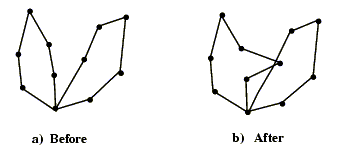
\includegraphics[width=10cm]{./fig/BreedSR.png}
\end{figure}


\item String Mix (SM): O melhor movimento entre SE e SR é selecionado.

 Para avaliar estes movimentos, Van Breedam considerou duas estratégias de melhoria local:

\begin{enumerate}
\item First Improvement (FI): Consiste de implementar o primeiro movimento que melhora a função
objetivo.
\item Best Improvement (BI): Avalia todas os possiveis movimentos e implementa o melhor destes.

 Van Breedam então define um conjunto de paramentros que pode influenciar o comportamento da
produção da melhoria local:

\begin{itemize}
\item A solução inicial (pobre, bom)
\item O comprimenro da string ($k$) para movimentos do tipo SE, SR, SM ($k$=1 ou 2)
\item A estratégia de selação (FI, BI)
\item O processo de avaliação para uma string de comprimento $k>1$ (avaliar todas as possiveis
strings de comprimento entre um de rotas, crescentod $k$ quando uma avaliação de ciclo inteiro tem
sido completado sem identificar um mevimento de melhoria).
\end{itemize}

\end{enumerate}

\end{enumerate}

\subsection{KINDERWATER AND SAVELSBERGH}

 Na heuristica de  Kinderwater e Savelsbergh rotas não são isoladas, então caminhos e clientes são
mudados entre diferêntes rotas. A operação que faz essas mudanças são:

\begin{enumerate}
\item Customer Relocation: Um cliente localizado em uma rota é mudado para outra

\begin{figure}[!ht]
\centering
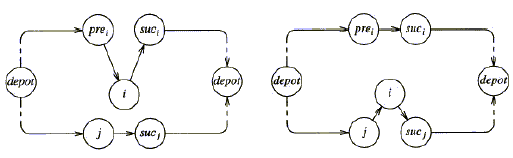
\includegraphics[width=10cm]{fig/KindSavCR.png}
\end{figure}

\item Crossover: Duas rotas são misturadas em um ponto

\begin{figure}[!ht]
\centering
\includegraphics[width=10cm]{fig/KindSavC.png}
\end{figure}

\item Customer Exchamge: Dois clientes de ruas rotas diferêntes são mudados entre duas rotas

\begin{figure}[!ht]
\centering
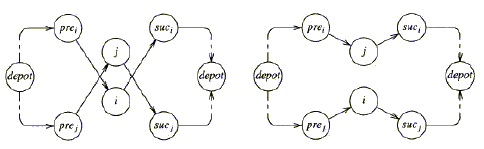
\includegraphics[width=10cm]{fig/KindSavCE.png}
\end{figure}
\end{enumerate}

 Nas figuras seguintes podemos ver um exemplor um pouco mais complexo:

\begin{figure}[!ht]
\centering
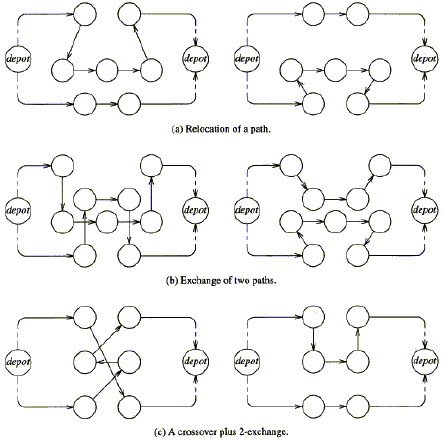
\includegraphics[width=10cm]{fig/KindSav.png}
\end{figure}





\chapter{Algoritmos de dois passos}
\section{Clark and Wright}

 O algoritmo econômia de Clarke e Wright é uma das mais conhecidas heuristicas para VRP. Foi
desenvolvido em {\color{red} referenciar} e aplica-se a problemas para os quais o numero de veículo
não é fixo, e trabalha igualmente bem para problemas com digrafos e grafos. Quando duas rotas
$(0,\ldots, i, 0)$ e $(0,j,\ldots,0)$ podem possivelmente ser mescladas em uma rota simples
$(0,\ldots,i,j,\ldots,0)$, uma economia de distância $s_{ij}=c_{i0}+c_{0j}-c_{ij}$ é gerada. O
algoritmo trabalha como segue:

\begin{description}
\item[Step 1.] Savings computation

\begin{itemize}
\item Calcule o custo $s_{ij} = c_{i0}+c_{0j}-c_{ij}$ para $i,j=1,\ldots,n$ e $i\neq j$.
\item Crie $n$ rotas de veículos $(0,i,0)$ para $i=1,\ldots,n$.
\item Ordene as poupanças de modo não crescente ( Não é necessário )
\end{itemize}

\item[Step 2.] Melhor combinação possivel

Inicie do topo da lista de custos, executando o seguinte:

\begin{itemize}
\item Dada um custo $s_{ij}$, determine se há duas rotas que podem possivelmente ser mescladas:

\begin{itemize}
\item Uma iniciando com $(0,j)$
\item Uma terminando com $(0,i)$
\end{itemize}

\item Combine essas duas rotas deletando $(0,j)$ e $(0,i)$ e introduzindo $(i,j)$.
\end{itemize}
%
%\item[Step 2.] Extensão de Rotas (Versão Sequêncial)
%\begin{itemize}
%\item Considere uma volta de cada rota $(0,i,\ldots,j,0)$.
%\item Determine a primeira poupança $s_{ki}$ ou $s_{jl}$ que pode possivelmente ser usada para
%mesclar a rota atual com outra rota terminando com $(k,0)$ ou iniciando com $(0,l)$.
%\item Implemente a mescla e repetição dessa operação para a rota atual.
%\item Se não há mesclas possiveis, considere a próxima rota e reaplique a mesma operação.
%\item Pare quando a mesclagem de rotas não for possivel.
%\end{itemize}

\end{description}

\section{Emparelhamento baseado no algoritmo de poupança}

 Ista é uma modificação interessante para o algoritmo de poupança padrão ( descrições similares são
feitas por {\color{red} referênciar} e {\color{red} referênciar} onde em cada interação a poupança
$s_{ij}$ obtida por mesclar rotas $p$ e $q$ é calculado como $s_{ij} = t(S_i) + t(S_j) - t(S_i \cap
S_j)$, onde $S_k$ é o conjunto de vértices da rota k, e $t(S_k)$ é o comprimento de uma solução
ótima para o TSP em $S_k$.

 Um problema de emparelhamento sobre o conjunto $S_k$ é resolvido usando os $s_{ij}$ valores com
custo de emparelhamento, e as rotas correspondem à emparelhamento ótimo estão mescladas a
permanencia da fazibilidade.


\section{Algoritmo de melhoria para Mult-rota}

 Algoritmos de melhoria esforçam-se para atualizar alguma possivel solução executando um sequência
de mudançãs dos vertices e arestas dentro ou entre rotas de veículos. Heuristicas de melhoramento de
multi-rotas para VRP operão em cada rota de veículo tomando muitas rotas em um tempo(?). Podemos
encontrar descrições de mudanças de arestas para VRP nestas três referências:

\begin{itemize}
\item {\color{red} Referenciar}
\item {\color{red} Referenciar}
\item {\color{red} Referenciar}
\end{itemize}

 Thompson e Psaraftis (1993) propõem um método baseado nos conceitos de $k$-transferência ciclicas
que envolvem transferência de $k$ demandas da rota $I^j$ para a rota $I^{\delta(j)}$ para cada $j$ e
inteiro fixo $k$. O conjunto de rotas $\{ I^r \}$, com $r = 1, \ldots, m$, constitui um solução
possivel e $\delta$ é uma permutação cíclica de um subconjunto de $\{1, \ldots, m\}$. Em particular,
quando $\delta$ tem cardinalidade fixa $C$, obtemos um $C$-ciclo $k$-transferência. Permitindo $k$
demanda modelo em cada rota, transferência de demanda pode ser realizada através de permutações mais
que permutações ciclicas, Devido a complexidade das pesquisas de vizinhanças de transferências
cíclicas, é realizada heuristicamente. O operador de 3-ciclo 2-transferências é ilustrado na figura
abaixo.


\begin{figure}[!ht]
\centering
\includegraphics[width=10cm]{./fig/thompPsar.png}
\caption{O operador de transferência cíclica. A ideia base é transferir simultaneamente os clientes
denotados pelo ciclo branco de maneira ciclica entre as rotas. Mais precisamente aqui clientes $a$ e
$c$ na rota 1, $f$ e $j$ na rota 2 e $o$ e $p$ na rota 4 são transferidos simultaneamente para as
rotas 2, 4, e 1 respectivamente e a rota 3 permanece intocada.}
\end{figure}

\subsection{VAN BREEDAM'S ANALYSIS}

 Agora sumarizaremos a analise de Van Breedam's. Há quatro operações a considerar, as quais são:

\begin{enumerate}
\item String Cross (SC): Duas cadeias de vertices são mudadas pelo cruzamento de duas arestas de
diferêntes rotas.

\begin{figure}[!ht]
\centering
\includegraphics[width=10cm]{./fig/BreedSC.png}
\end{figure}

\item String Exchange (SE): Duas cadeias de no mínimo $k$ vértices são mudadas entre duas rotas.

\begin{figure}[!ht]
\centering
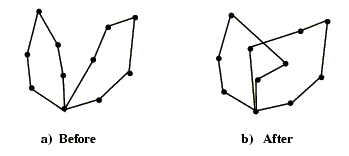
\includegraphics[width=10cm]{./fig/BreedSE.png}
\end{figure}

\item String Realocação (SR): Uma cadeia de no mínimo k vertices é deslocada de uma rota para outra,
tipicamente com $k=1$ ou 2.

\begin{figure}[!ht]
\centering
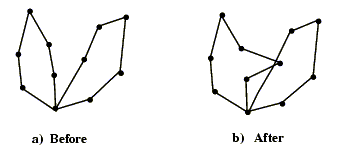
\includegraphics[width=10cm]{./fig/BreedSR.png}
\end{figure}


\item String Mix (SM): O melhor movimento entre SE e SR é selecionado.

 Para avaliar estes movimentos, Van Breedam considerou duas estratégias de melhoria local:

\begin{enumerate}
\item First Improvement (FI): Consiste de implementar o primeiro movimento que melhora a função
objetivo.
\item Best Improvement (BI): Avalia todas os possiveis movimentos e implementa o melhor destes.

 Van Breedam então define um conjunto de paramentros que pode influenciar o comportamento da
produção da melhoria local:

\begin{itemize}
\item A solução inicial (pobre, bom)
\item O comprimenro da string ($k$) para movimentos do tipo SE, SR, SM ($k$=1 ou 2)
\item A estratégia de selação (FI, BI)
\item O processo de avaliação para uma string de comprimento $k>1$ (avaliar todas as possiveis
strings de comprimento entre um de rotas, crescentod $k$ quando uma avaliação de ciclo inteiro tem
sido completado sem identificar um mevimento de melhoria).
\end{itemize}

\end{enumerate}

\end{enumerate}

\subsection{KINDERWATER AND SAVELSBERGH}

 Na heuristica de  Kinderwater e Savelsbergh rotas não são isoladas, então caminhos e clientes são
mudados entre diferêntes rotas. A operação que faz essas mudanças são:

\begin{enumerate}
\item Customer Relocation: Um cliente localizado em uma rota é mudado para outra

\begin{figure}[!ht]
\centering
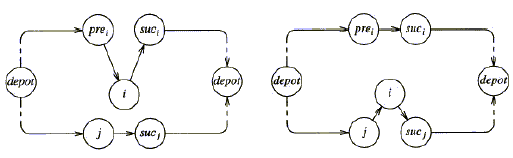
\includegraphics[width=10cm]{fig/KindSavCR.png}
\end{figure}

\item Crossover: Duas rotas são misturadas em um ponto

\begin{figure}[!ht]
\centering
\includegraphics[width=10cm]{fig/KindSavC.png}
\end{figure}

\item Customer Exchamge: Dois clientes de ruas rotas diferêntes são mudados entre duas rotas

\begin{figure}[!ht]
\centering
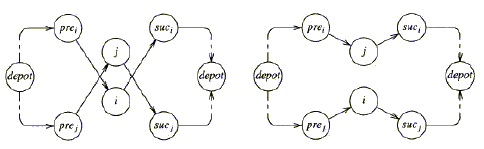
\includegraphics[width=10cm]{fig/KindSavCE.png}
\end{figure}
\end{enumerate}

 Nas figuras seguintes podemos ver um exemplor um pouco mais complexo:

\begin{figure}[!ht]
\centering
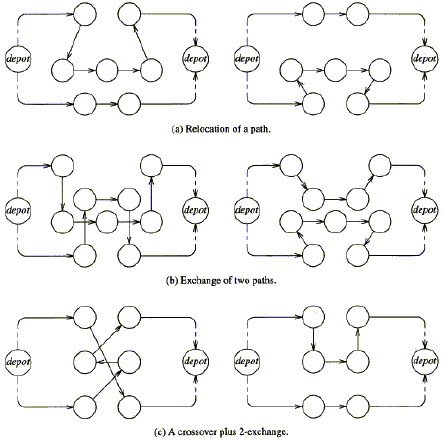
\includegraphics[width=10cm]{fig/KindSav.png}
\end{figure}




\end{document}
